%% Draft settings
\documentclass[10pt]{article}
\usepackage{amsmath}
\usepackage{amssymb}
\usepackage{graphicx}
\usepackage{subfigure}
\usepackage{color}
 \usepackage{lineno}
\usepackage{simplemargins}
\usepackage{natbib}

% \linenumbers*[1]
 \usepackage[T1]{fontenc} % For citing barki{\dj}ija
\setkeys{Gin}{draft=false}


% Margins
\setleftmargin{1in}
\setrightmargin{1in}
\setbottommargin{1in}
\settopmargin{1in}
 
% My Commands
%\input{tensor_book_shrtcts.tex}
\newcommand{\comment}[1]{\textcolor{blue}{[{#1}]}}


%%Nadir's Shortcuts
\newcommand{\beqn}{\begin{equation}}
\newcommand{\eeqn}{\end{equation}}
\newcommand{\beqa}{\begin{eqnarray}}
\newcommand{\eeqa}{\end{eqnarray}}
\newcommand{\beqanonum}{\begin{eqnarray*}}
\newcommand{\eeqanonum}{\end{eqnarray*}}
\newcommand{\beqnonum}{\begin{equation*}}
\newcommand{\eeqnonum}{\end{equation*}}
\newcommand{\jump}{\vspace{0.5cm}}
\newcommand{\bbf}{\begin{bf}}
\newcommand{\ebf}{\end{bf}}
\newcommand{\eqnref}[1]{(\ref{#1})}
\newcommand{\defn}[1]{\begin{bf}\emph{#1}\end{bf}}
\newcommand{\reals}{\ensuremath{\mathbb{R}}}
\newcommand{\complex}{\ensuremath{\mathbb{C}}}
\newcommand{\integers}{\ensuremath{\mathbb{Z}}}
\newcommand{\half}{\ensuremath{\frac{1}{2}}}
\newcommand{\n}{\nonumber}
\newcommand{\inverse}{^{-1}}

%calculus shorthand
\newcommand{\timeder}{\frac{d}{dt}}
\newcommand{\partialder}[1]{\frac{\partial}{\partial #1}}
\newcommand{\partialderf}[2]{\ensuremath{\frac{\partial #1}{\partial #2}}}
\newcommand{\der}[2]{\ensuremath{\frac{d #1}{d #2}}}
\newcommand{\dx}{\ensuremath{\frac{d}{dx}}}
\newcommand{\ddx}{\ensuremath{\frac{d}{dx}}}
\newcommand{\kvec}{\ensuremath{\vec{k}}}
\newcommand{\uvec}{\ensuremath{\mathbf{u}}}
\newcommand{\zhat}{\ensuremath{\mathbf{\hat{z}}}}
\newcommand{\khat}{\ensuremath{\mathbf{\hat{k}}}}
\newcommand{\unitvect}[1]{\ensuremath{\mathbf{\hat{#1}}}}
\newcommand{\ppx}{\ensuremath{\partial_x}}
\newcommand{\ppy}{\ensuremath{\partial_y}}
\newcommand{\ppz}{\ensuremath{\partial_z}}
\newcommand{\ppt}{\ensuremath{\partial_T}}
\newcommand{\ppp}{\ensuremath{\partial_p}}


% radiation shorthand
\newcommand{\cotwo}{\ensuremath{\mathrm{CO_2}}}
\newcommand{\othree}{\ensuremath{\mathrm{O_3}}}
\newcommand{\htwo}{\ensuremath{\mathrm{H_2O}}}
\newcommand{\QLW}{\ensuremath{Q_\mathrm{LW}}}
\newcommand{\QSW}{\ensuremath{Q_\mathrm{SW}}}
\newcommand{\Qnet}{\ensuremath{Q_\mathrm{net}}}
\newcommand{\FLW}{\ensuremath{F^\mathrm{LW}}}
\newcommand{\FSW}{\ensuremath{F^\mathrm{SW}}}
\newcommand{\FLWgl}{\ensuremath{F^\mathrm{LW}_{\mathrm{gl}}}}
\newcommand{\FSWgl}{\ensuremath{F^\mathrm{SW}_{\mathrm{gl}}}}
\newcommand{\USW}{\ensuremath{U^\mathrm{SW}}}
\newcommand{\DSW}{\ensuremath{D^\mathrm{SW}}}
\newcommand{\Fnet}{\ensuremath{F^\mathrm{net}}}
\newcommand{\Fnetgl}{\ensuremath{F^\mathrm{net}_{\mathrm{gl}}}}
\newcommand{\Fgl}{\ensuremath{F_{\mathrm{gl}}}}
\newcommand{\olr}{\ensuremath{\mathrm{OLR}}}
\newcommand{\OLR}{\ensuremath{\mathrm{OLR}}}
\newcommand{\trans}{\ensuremath{\mathcal{T}}}
\newcommand{\solar}{\ensuremath{I_0}}
\newcommand{\cool}{\ensuremath{\mathcal{C}}}
\newcommand{\cminverse}{\ensuremath{\mathrm{cm^{-1}}}}
\newcommand{\pierre}{P10}
\newcommand{\tauk}{\ensuremath{\tau_k}}
\newcommand{\Wmsq}{\ensuremath{\mathrm{W/m^2}}}

% meteorology shorthand
\newcommand{\qv}{\ensuremath{q}}
\newcommand{\rhov}{\ensuremath{\rho_\mathrm{v}}}
\newcommand{\Hv}{\ensuremath{H_\mathrm{v}}}
\newcommand{\Rv}{\ensuremath{R_\mathrm{v}}}
\newcommand{\qa}{\ensuremath{q_a}}
\newcommand{\qvstar}{\ensuremath{q^*}}
\newcommand{\Ta}{\ensuremath{T_a}}
\newcommand{\Tav}{\ensuremath{T_\mathrm{av}}}
\newcommand{\Ts}{\ensuremath{T_\mathrm{s}}}
\newcommand{\Tsgl}{\ensuremath{T_\mathrm{s,gl}}}
\newcommand{\ps}{\ensuremath{p_s}}
\newcommand{\RH}{\ensuremath{\mathrm{RH}}}
\newcommand{\cld}{\ensuremath{\mathrm{Cld}}}
\newcommand{\WVP}{\ensuremath{\mathrm{WVP}}}
\newcommand{\ztop}{\ensuremath{z_\mathrm{top}}}
\newcommand{\ztp}{\ensuremath{z_\mathrm{tp}}}
\newcommand{\zlcl}{\ensuremath{z_\mathrm{LCL}}}
\newcommand{\Tlcl}{\ensuremath{T_\mathrm{LCL}}}
\newcommand{\Ttp}{\ensuremath{T_\mathrm{tp}}}
\newcommand{\ptp}{\ensuremath{p_\mathrm{tp}}}
\newcommand{\lapseav}{\ensuremath{\Gamma_\mathrm{av}}}
\newcommand{\gammaav}{\ensuremath{\Gamma_\mathrm{av}}}
\newcommand{\Kinverse}{\ensuremath{\mathrm{K^{-1}}}}
\newcommand{\Htauk}{\ensuremath{H_{\tau_k}}}
\newcommand{\east}{\ensuremath{\mathrm{E}}}
\newcommand{\north}{\ensuremath{\mathrm{N}}}
\newcommand{\south}{\ensuremath{\mathrm{S}}}
\newcommand{\tav}{\ensuremath{t_\mathrm{av}}}

%Variables
\newcommand{\figurepath}{../figures/}


\begin{document}

%% ------------------------------------------------------------------------ %%
%
%  TITLE
%
%% ------------------------------------------------------------------------ %%


\title{Invariant Radiative Cooling and Mean Precipitation Change}

%% ------------------------------------------------------------------------ %%
%
%  AUTHORS AND AFFILIATIONS
%
%% ------------------------------------------------------------------------ %%


 \author{Nadir Jeevanjee\footnote{Department of Physics, University of California at Berkeley, Berkeley, CA 94702  USA. jeevanje@berkeley.edu (corresponding author)} \footnote{Climate and Ecosystems Science Division, Lawrence Berkeley National Laboratory, Berkeley, CA USA} and David Romps\footnote{Department of Earth and Planetary Sciences, University of California at Berkeley, Berkeley, CA 94702  USA.} \footnote{Climate and Ecosystems Science Division, Lawrence Berkeley National Laboratory, Berkeley, CA USA}
}

\maketitle

\begin{abstract}
We show that radiative cooling profiles,  when described in temperature  coordinates, are insensitive to surface temperature \Ts. This \Ts-invariance is a result of water vapor's dominance as both a greenhouse gas and sunlight absorber, as well as its density being tightly constrained by the Clausius-Clapeyron equation. As such, \Ts-invariance holds for the shortwave and longwave channels separately, as well as together. Furthermore, the \Ts-invariance of vertically-resolved cooling profiles leads to simple expressions for the \Ts-dependence of column-integrated cooling and hence precipitation, and gives insight into why mean precipitation increases at a rate of $O(1\%)\ \Kinverse$.  Our results are tested against cloud-resolving simulations of the tropical atmosphere. We also assess the relevance of our results to global climate simulations.
%\vspace{0.5cm}
%
%
\end{abstract}


%% ------------------------------------------------------------------------ %%
%
%  TEXT
%
%% ------------------------------------------------------------------------ %%


\section {Introduction}
Despite its fundamental role in driving atmospheric motions, atmospheric radiative cooling remains somewhat enigmatic. Though the fundamentals of radiative transfer are quite well-understood and have been for some time, translating these fundamentals into realistic cooling rates requires a symphony of complicated spectroscopic and radiative transfer calculations which render the final result somewhat inscrutable. As a result, we lack simple descriptions of the radiative cooling profiles produced by our numerical models.

%  calculating highly frequency-dependent optical depth profiles from the molecular spectroscopy of the various radiatively active gases, solving the radiative transfer equations for both upwelling and downwelling fluxes separately, differentiating in the vertical to get a spectral cooling rate, and finally integrating across frequency space to get the total cooling rate. By the time this is done most intuition that one has from simple, textbook gray-body calculations is lost, and we lack any simple descriptions of the resulting realistic but physically opaque cooling profiles.

One implication of this is that quantities that are closely tied to radiative cooling, such as global mean precipitation, also remain somewhat enigmatic. We do know that the atmospheric (rather than planetary) energy budget, in which condensation heating from precipitation balances atmospheric radiative cooling, constrains global mean precipitation $P$ to be roughly equal to column-integrated net radiative cooling $\Qnet$ \citep{ogorman2012,allen2002}:
\beqn
	LP = \Qnet \quad \mbox{(\Wmsq)} \label{rad_precip_constraint}
\eeqn
(here $L$ is the latent heat of vaporization). We also know that both cloud-resolving models and global climate models robustly exhibit  mean precipitation increases with warming of $O(1\%)\ \Kinverse$  \citep{stephens2008, lambert2008, held2006}. \comment{read and cite lambert2008b?}. What's more, \cite{pendergrass2014} recently explained this increase in global mean precipitation in terms of an increase in downward radiative emission from the atmosphere at the surface. Despite this progress, however, a basic question remains unanswered: why does this increase takes on the value that it does? Why $O(1\%)\ \Kinverse$, and not an order of magnitude larger or smaller?

This paper aims to reveal some simple behavior in radiative cooling profiles, and to use it to try and answer this question about precipitation change. The physics we rely on is not new, but was rather noted as far back as \cite{simpson1928}, and revived recently by \cite{ingram2010}. Our contribution here is to shift the focus from outgoing longwave radiation to atmospheric radiative cooling, and to extend the argument to both the longwave (LW) and shortwave (SW) channels. 

We will  focus on how vertically-resolved radiative cooling profiles change with warming, rather than focusing on radiative fluxes at the surface or TOA as in \cite{pendergrass2014}. In particular, we will argue, following \cite{simpson1928} and \cite{ingram2010}, that water vapor density and optical depth profiles should behave very simply when considered as functions of temperature as a vertical coordinate. This then implies almost immediately that LW and SW radiative flux divergences should also behave simply in temperature coordinates. This simple behavior leads to prognostic expressions for $d\Qnet/d\Ts$ and hence $dP/d\Ts$, which we validate with a cloud-resolving model (CRM). We then extend our results from CRMs to global climate models (GCMs),  and seek insight from our formulae which apply in both contexts. 


\section{CRM Simulations of RCE}
We begin by studying precipitation change in one of the simplest systems in which the radiative constraint on precipitation \eqnref{rad_precip_constraint} operates, namely tropical oceanic radiative-convective equilibrium (RCE) with fixed sea-surface temperature. This system approximates the real tropics, where the majority of Earth's precipitation occurs \citep{simpson1988}, and like the GCMs exhibits precipitation increases of roughly $O(1\%)\ \Kinverse$ \citep{romps2011, muller2011b}.  

We simulate RCE using Das Atmosph\"arische Modell \citep[DAM,][]{romps2008},   a three-dimensional, fully-compressible, non-hydrostatic cloud-resolving model, coupled to radiation via the Rapid Radiative Transfer Model 
\citep[RRTM,][]{mlawer1997}. DAM employs the six-class Lin-Lord-Krueger  microphysics scheme \citep{lin1983, lord1984, krueger1995}, and relies on implicit LES \citep{margolin2006} for sub-grid scale transport, so no explicit sub-grid scale turbulence scheme is used.
	
	Our RCE simulations ran on a square doubly-periodic domain of horizontal dimension $L=72$ km, with  a horizontal resolution of $dx=1$ km. The vertical grid stretched smoothly from 50 m resolution below 1000 m to 250 m resolution between 1000 m and 5000 m, and then to 500 m up to the model top at  30 km. We calculated surface heat and moisture fluxes using a bulk aerodynamic formula, and used a pre-industrial \cotwo\  concentration of 280 ppm with no ozone except where specified otherwise. To explore precipitation changes  with warming we ran four experiments at surface temperatures of $\Ts=(280,290,300,310)$ K. Our runs branched off the equilibrated runs described in \cite{romps2014}, and were run for 60 days  to iron out any artifacts from changing the domain and resolution. All vertical profiles are time-mean and domain-mean, averaged over the last 20 days of each run. 

Since we run with prescribed \Ts, our warming experiments are somewhat artificial, in that the warming is not driven by increases in \cotwo. This has the advantage that we isolate part of the physics and thus have a better chance at arriving at a simple description, but has the disadvantage that we omit the direct effect of increased \cotwo\ on atmospheric cooling and hence precipitation, an effect of roughly -1 \Wmsq/K. This omission does not affect our main conclusions about precipitation change, however, as we will see later on.

%=================================%
% Temperature invariance of flux divergence %
%=================================%
\section{\Ts-invariance of Flux Divergences}
The simple behavior of radiative cooling alluded to above begins with the key fact that  the water vapor density 
	\beqn
		\rhov =  \RH\frac{p_v^*(T)}{R_ vT} \; 
	\label{rhov}
	\eeqn
	 is (up to variations in relative humidity \RH) a function of temperature only.\footnote{Here $p_v^*$  is the saturation vapor pressure of water, and all other symbols have their usual meaning.} If we use $T$ as a vertical coordinate,  Eqn. \eqnref{rhov} then tells us that the function $\rhov(T)$ does not depend on \Ts. This is what we mean by `\Ts-invariance'. We verify \Ts-invariance of $\rhov(T)$  in Fig. \ref{rhov_fig}, where indeed  the \rhov\ profiles at different \Ts\ collapse onto a single curve when plotted in temperature coordinates.
	 
	For wavenumbers $k$ outside of spectral bands where other trace gases (like \cotwo\ and \othree) dominate, the optical depth $\tauk$ is just
	\beqn
		\tau_k(z) = \int_z^\infty \kappa(k)  \rhov(z') \, dz'  \; 
		\label{tauz}
	\eeqn
		where $\kappa(k)$ is a  mass absorption coefficient  (units $\mathrm{m^2/kg}$) whose pressure-broadening and temperature scaling we neglect. Changing the integration variable to temperature $T'$ yields
		\beqn
		\tau_k(T) = \int_{\Ttp}^T \kappa(k)  \rhov(T') \, \frac{dT'}{\Gamma}  \; ,
		\label{tauT}
	\eeqn
	where we neglect stratospheric water vapor and take the lower limit of the integral to be the tropopause temperature $\Ttp \approx 185$ K, where radiative cooling goes to 0 (see Figs. \ref{pptflw_tinv_dam} and  \ref{pptfsw_tinv_dam}, which also show that \Ttp\ is \Ts-invariant). The only quantity in Eqn. \eqnref{tauT} which might still exhibit some \Ts-dependence is the  moist lapse rate $\Gamma$, but Figure 2 of \cite{ingram2010} shows that when $\Gamma$ is considered a function of temperature, it too is fairly  \Ts-invariant. Equation \eqnref{tauT} then implies that \tauk\ profiles at any $k$ exhibit the same \Ts-invariance as \rhov. This argument was also made by \cite{ingram2010}, and its essence goes back to  \cite{simpson1928}.
	
	To connect all this with radiative cooling, we invoke the cooling-to-space (CTS) approximation \citep[e.g.,][]{thomas2002}, which says that the spectrally resolved LW flux divergence in temperature coordinates $-\ppt \FLW_k$ (units $\Wmsq/\mathrm{K}/\cminverse$, minus sign introduced to maintain a consistent sign with  $\ppz \FLW_k$) is approximately
	\beqn
		-\ppt \FLW_k \approx - \pi B_k(T) \frac{d (e^{-\tauk(T)})}{dT}
	\label{cts_spectral}
	\eeqn
where  the transmission function $e^{-\tauk}$ gives the fraction of radiation emitted at a given height which travels unabsorbed out to space. Since the Planck function $B_k(T)$ is \Ts-invariant, and $\tauk(T)$ is as well, we also expect $-\ppt \FLW_k$ to be \Ts-invariant. Since this holds for all $k$ where water vapor dominates, it should also hold approximately for the spectrally integrated LW flux divergence $-\ppt \FLW$ ($\Wmsq/\mathrm{K}$). This is confirmed in  Fig.  \ref{pptflw_tinv_dam}, which plots $(-\ppt \FLW)(T)$ as diagnosed from RRTM coupled to our  RCE simulations.  That figure also plots $-\ppt \FLW$ as functions of $z$ and $p$, to emphasize that this invariance only holds  when $T$ is used as the vertical coordinate.
	
	A similar argument holds for the shortwave (SW) flux divergence. If $I_k$ is the incident solar flux at wavenumber $k$, and  neglecting reflection and scattering in the  near-infrared, 
%\citep[e.g.][]{frouin1990}, 
then without further approximation we have
	\beqn
		-\ppt \FSW_k = - I_k \der{(e^{-\tauk(T)})}{T}
		\
	\eeqn
\citep[c.f.][eqn. 9.26]{thomas2002}. This equation is similar to  \eqnref{cts_spectral} but with $B_k(T) \rightarrow I_k$, and since $I_k$ is also \Ts-invariant, we can argue as above that $(-\ppt \FSW)(T)$ should be \Ts-invariant. This is confirmed in Fig. \ref{pptfsw_tinv_dam}, where again the simple behavior of $-\ppt \FSW$ in temperature coordinates is contrasted with that in height and pressure coordinates.

The fluxes used in Figs.  \ref{pptflw_tinv_dam} and \ref{pptfsw_tinv_dam} are all-sky fluxes, but the foregoing argument was for clear-sky fluxes. This is permissible because cloud fractions in our RCE simulations are low (attaining a maximum of $\sim 10 \%$ at the anvil height in our simulations), so it is the clear-sky physics which dominates. We will return to atmospheric cloud radiative effects in section \ref{sec_GCMs}, when we extend this framework to GCMs.
 
%=================%
% Simple picture for Q   %
%=================%
		
\section{A simple picture for column-integrated radiative cooling} \label{sec_simple_Q}

Now that we have established  the \Ts-invariance of radiative flux divergences, we can construct a simple, quantitative picture of how column-integrated radiative cooling, and hence precipitation,  changes with surface temperature. 
	
	Let $F$ denote radiative flux in a particular channel -- LW, SW, or Net (LW+SW) -- and $Q$ the associated column-integrated free-tropospheric radiative cooling. We consider  the free troposphere, rather than the full troposphere, because the radiative constraint on precipitation 
		\beqn
			P \approx \Qnet
		\label{p_constraint}
		\eeqn
		 (where we now absorb a factor of $L$ into $P$) holds best for the free troposphere  \citep{ogorman2012}. We define the free troposphere here as being above the lifting condensation level \Tlcl\ and below the tropopause \Ttp.
	
	  The basic idea is to write $Q$ as an integral of $-\ppt F$  in temperature coordinates: 
	\beqn
		Q =  \int_{\Ttp}^{\Tlcl} (-\partial_{T'} F) dT' \ . 
		\n
	\eeqn
   If we approximate the change in  \Tlcl\ as equal to the change in \Ts, then the change in $Q$ with surface temperature is  simply
	\beqn
		\der{Q}{\Ts} \ =\  \left.  -\ppt F\right|_{\Tlcl}  \; .
	\label{dqdts}
	\eeqn
In other words, since the tropospheric cooling profile $(-\ppt F)(T)$  is independent of \Ts, increasing \Ts\ just exposes more of this profile.  The contribution of this new section of the $(-\ppt F)(T)$ curve to $Q$ is given by \eqnref{dqdts}.  A cartoon of this argument is given in Fig. \ref{dqdts_cartoon}. For finite changes in \Ts, Eqn. \eqnref{dqdts} approximates $(-\ppt F)(T)$ in the newly exposed region as equal to $-\ppt F$ at the LCL of the base state, but for small enough changes in \Ts\ this approximation should be adequate. Specializing Eqn. \eqnref{dqdts} to the Net channel and invoking \eqnref{p_constraint} then yields a \emph{prognostic} equation for precipitation change with surface warming.

Let us test the predictive power of Eqn. \eqnref{dqdts}. The panels of Fig. \ref{Qnet_varsst} plot $Q(\Ts)$ as diagnosed directly from our CRM simulations, along with estimates of the slope of this curve diagnosed via  Eqn. \eqnref{dqdts}, for the SW, LW, and Net  channels (\Tlcl\ is diagnosed as $T$ at the low-level maximum in cloud fraction). Precipitation $P$ is also plotted alongside $\Qnet$.  Figure \ref{Qnet_varsst} shows that  Eqn. \eqnref{dqdts}  captures the changes in  cooling in all channels. Furthermore, since $P$ tracks \Qnet\ closely for $290\leq \Ts \leq 310$ K, Eqn. \eqnref{dqdts} also captures precipitation changes, at least in this temperature regime.

We also see that  Eqn. \eqnref{dqdts} predicts a \emph{decrease} in  \Qnet\ with \Ts\ at \Ts=320 K; this is not an error in our diagnostic equation \eqnref{dqdts} , but rather a real effect due to the fact that $-\ppt \FLW$ tends towards zero with increasing $T$,\footnote{We speculate that runaway greenhouse physics, known to set in at roughly 310 K \citep{goldblatt2013}, is responsible for this behavior, but leave detailed investigation of this to future work.} while -\ppt \FSW\ is staying roughly constant. This leads to radiative heating, rather than cooling, in the  lower troposphere, which violates the basic radiative-convective paradigm; it is perhaps then no surprise that the constraint \eqnref{p_constraint} appears to break down in this \Ts\ regime. The radiative constraint on precipitation also breaks down for $\Ts \leq 280$ K, where sensible heat fluxes start to dominate over latent heat fluxes. Thus, Eqn. \eqnref{dqdts} has explanatory power for  precipitation changes at  temperatures somewhat greater than or equal to Earth's mean temperature of 288 K, but outside the $290\leq \Ts \leq 310$ K range, other constraints besides our purely radiative one seem to be required to predict changes in $P$.

%===========%
% Why 1%/K?    %		
%===========%

\section{Why does precipitation increase at $O(1\%)\ \Kinverse$?} \label{sec_1percent}
The results in Fig. \ref{Qnet_varsst} show that our framework  has some predictive power for explaining changes in \Qnet\ and hence $P$. Let us then try to use this framework to answer the question posed in the introduction, namely: why does mean precipitation increase at $O(1\%)\ \Kinverse$?

First, let us confirm in a back-of-the-envelope fashion that Eqn. \eqnref{dqdts} indeed gives a $O(1\%)\ \Kinverse$ increase in $P$. Combining \eqnref{p_constraint} and \eqnref{dqdts} gives
	\beqn
		\frac{d \ln  P}{d \Ts} \ \approx\  \frac{(-\ppt \Fnet)(\Tlcl)}{\Qnet} \; .
	\label{precip_estimate}
	\eeqn
For \Ts=300 K, where $(-\ppt \Fnet)(\Tlcl) \approx 3 \ \Wmsq/\mathrm{K}$ and $\Qnet =  104\ \Wmsq$, we find $\frac{d \ln  P}{d \Ts}=  3\%\ \Kinverse$, which is indeed  $O(1\%)\ \Kinverse$.

Now, suppose we take \Ts=300 K and  try to simply parametrize the net cooling as $-\ppt \Fnet \sim (T-\Ttp)^\beta$. We ignore any proportionality constant out front, and further suppose (motivated by inspection of Figs. \ref{pptflw_tinv_dam} and \ref{pptfsw_tinv_dam})  that $\beta \approx 1$, i.e. that $-\ppt \Fnet$ is roughly linear in $(T-\Ttp)$. Then the full tropospheric radiative cooling is $Q\sim (\Ts-\Ttp)^{\beta+1}$, and hence 
	\beqn
		\frac{d \ln Q}{d \Ts}  =  \frac{\beta+1}{\Ts-\Ttp}\ . \label{dqdts_approx}
	\eeqn
Note that $\Ts-\Ttp$ is the \emph{depth of the troposphere expressed in temperature coordinates}. For  \Ts= 300 K this depth is roughly 100 K, and so \eqnref{dqdts_approx} gives roughly 2 \% \Kinverse, which is again $O(1\%)\ \Kinverse$.

Now, further suppose that $-\ppt \Fnet$ were constant throughout the depth of the troposphere, i.e. $\beta=0$. Then $Q$ would just scale with $\Ts-\Ttp$. But then it is clear that, since \emph{a 1 K increase in \Ts\  is a $1\%$ increase in tropospheric depth \Ts-\Ttp}, $Q$ should increase at 1 \% \Kinverse. The fact that Q increases slightly faster than that can then be understood as a result of the fact that $-\ppt \Fnet$ is increasing, not constant, with $T$, i.e. that $\beta$ in \eqnref{dqdts_approx} is greater than 0.

%===========%
% GCMs            %		
%===========%

\section{Extension to GCMs} \label{sec_GCMs}
The framework presented so far has an appealing simplicity. But, the question remains as to whether our results, derived and tested in the context of highly idealized and horizontally homogenous RCE, hold up in comprehensive global climate models (GCMs). The most obvious extension of the foregoing results would be to apply them to GCMs on a column-by-column basis. As a first check, then, we should confirm that  for each latitude and longitude (collectively denoted  by a solid angle coordinate $\Omega$),  climatological  $(-\ppt F)(\Omega,T)$ profiles satisfy \Ts-invariance. 

For this we utilize the AMIP and AMIP4K  output in the CMIP5 archive. These experiments are atmosphere-only, and feature observed SSTs (AMIP) as well as uniform perturbations to those observed SSTs (AMIP4K), with no change in \cotwo\ concentration; as such they are good analogs to our CRM experiments. The AMIP4K experiment was part of the CFMIP protocol, which also requested the output of vertically-resolved radiative fluxes, rather than just surface and TOA fluxes, allowing us to compute $-\ppt F$ profiles.

Six models participated in the AMIP and AMIP4K CFMIP experiments and provided the output we require. We begin by analyzing one of them, HadGEM2-A. Plots of climatological $(-\ppt \Fnet)(T)$ for columns in the west Pacific warm pool, Pacific trade cumulus regime, and east Pacific cold tongue,  for both the AMIP and AMIP4K simulations, are shown in the top row of Fig. \ref{local_pptf_profiles} (see appendix for computational details). These panels show that while \Ts-invariance holds quite well in the upper troposphere, it fails in the lower troposphere, where many features move down to higher temperatures with surface warming. This stands in contrast to the CRM $(-\ppt F)(T)$ profiles, which under warming reach the new \Ts\ not by \emph{shifting} down but by \emph{extending} downward.
%sometimes revealing rather marked new features (such as the local minimum at $T=280$ K in -\ppt \FLW revealed by increasing \Ts\ from 280 to 290 K; Fig. \ref{pptflw_tinv_dam}).

Thus, the rationale underlying \eqnref{dqdts} fails. But, what about the qualitative conclusion from Section \ref{sec_1percent}, that $d\ln Q/d\Ts$ is $O(1\%)\ \Kinverse$ because a 1 K increase in \Ts\ is a 1\% increase in tropospheric depth? Could such an interpretation still somehow hold for GCMs, despite the apparent lack of \Ts-invariance?

The downward shift at higher temperatures of the $-\ppt \Fnet(T)$ profiles  in  Fig. \ref{local_pptf_profiles} point to a potential way forward. Such a shift seems consistent with the various local extrema of the profiles occurring at fixed lower-tropospheric pressure, rather than temperature. Indeed, investigations of the non-\Ts-invariance in Fig. \ref{local_pptf_profiles} suggest that lower-tropospheric local extrema in $-\ppt F$  arise from a variety of causes, including stratocumulus and trade cumulus clouds, temperature inversions, and especially sharp relative humidity gradients. Such features might be expected to stay closer to fixed pressure than fixed temperature with warming. This suggests that we find a coordinate that, with warming, behaves like temperature in the upper troposphere but like pressure in the lower troposphere. One such coordinate is the fractional temperature coordinate
\beqn
	\alpha \equiv \frac{T-\Ttp}{\Ts - \Ttp}\ ,
	\label{alpha_def}
\eeqn
where \Ts\ and \Ttp\ are column-dependent `surface' and tropopause temperatures. For each GCM column, $\alpha$ varies from 0 at the tropopause to 1 at the surface or tropospheric inversion, if present  (see appendix for details).

The bottom row of Fig. \ref{local_pptf_profiles} shows the same profiles as the top row, but plotted in $\alpha$ rather than $T$ coordinates. Use of the $\alpha$ coordinate significantly ameliorates the downward shift in the lower troposphere exhibited by the $(-\ppt \Fnet)(T)$ profiles (though there is a slight degradation of \Ts-invariance in the mid-troposphere in the eastern and western Pacific).  This suggests that \Ts-invariance in $\alpha$-coordinates, rather than $T$ coordinates, might be a viable way to understand radiative cooling and precipitation changes in a GCM.

The next question is whether \Ts-invariance in $\alpha$ coordinates is a reasonable approximation across the globe and across models. To proceed we average the $(-\ppt \Fnet)(\alpha)$ profiles over all columns to obtain a global average net flux divergence
	\beqn
		(-\ppt \Fnetgl)(\alpha) \equiv \frac{1}{4\pi\tav}\int_0^{\tav} dt \int d \Omega\  (-\ppt \Fnet)(\Omega,\alpha,t) \ .
		\label{pptfgl_def}
	\eeqn
The bottom row of Fig. \ref{local_pptf_profiles} suggests that these should be roughly \Ts-invariant. We confirm this  in Fig. \ref{pptfg_profiles}, which plots $-\ppt \Fnetgl(\alpha)$ for the AMIP and AMIP4K runs for all six our CFMIP models.  This plot shows that \Ts-invariance in $\alpha$ coordinates is indeed a reasonable approximation across the globe and across models. 

%The three models in the top row display good invariance in the upper and far lower troposphere, with  some increases in $-\ppt \FLWgl(\alpha)$ near $\alpha = 0.8$. (Such an increase is not surprising, since the temperature at fixed $\alpha$ increases with \Tsgl, and our CRM results show that $-\ppt \FLW$ generally increases with $T$.) The bottom row shows profiles for CanAM4, which displays excellent \Ts-invariance, and for  MPI-ESM-LR and MIROC5, whose $-\ppt \Fnetgl(\alpha)$ profiles exhibit a slight residual downward shift with warming.

% In particular, the AMIP and AMIP4K $-\ppt \FSWgl$ profiles collapse almost perfectly in $\alpha$ coordinates. The $-\ppt \FLWgl$ profiles do not collapse, however, as surface warming causes 

%The use of $\alpha$ coordinates thus seems to  yield a partial \Ts-invariance for this GCM; the location of local extrema in $(-\ppt \Fgl)(\alpha)$ seem to stay fixed, but there are potentially significant increases in $(-\ppt \FLWgl)(\alpha)$ which we cannot account for. Before exploring whether or not this partial \Ts-invariance can give us insight into why GCMs exhibit $O(1\%)\ \Kinverse$ increases in $Q$, we should first check how robust this \Ts-invariance is across models. 

Given this invariance, let us see to what degree it can help us understand the global cooling and precipitation changes exhibited by these models. To this end, we write the spatiotemporally varying, column-integrated radiative cooling $Q(\Omega,t)$ in $\alpha$ coordinates as 
	\beqn
		Q(\Omega,t)   =  \int_0^{1} (- \partial_{T} \Fnet) (\Ts - \Ttp)\, d\alpha  \ .
		\label{Q_alpha}
	\eeqn
Note the appearance of the local tropospheric depth in temperature coordinates, \Ts\ - \Ttp,  due to $dT/d\alpha$ computed from Eqn. \eqnref{alpha_def}. If we now assume that $\Ts(\Omega,t)$ scales directly with the global mean \Ts, the fractional increase in $Q(\Omega,t)$ with  warming is just 
\beqn
		\frac{d \ln Q(\Omega,t)}{d \Ts}  \ =\   \frac{1}{\Ts-\Ttp}\ . 
		\label{dqdts_gcm}
\eeqn
This equation is very similar to Eqn. \eqnref{dqdts_approx}, and thus  tells the  same basic story: in the present-day climate, a 1 K increase in \Ts\ amounts to a roughly 1\% increase in tropospheric depth,  and thus fractional changes in  $Q$ and $P$ are $O(1\%)\ \Kinverse$. 
%\Ts-invariance in $\alpha$ coordinates for GCMs tells us that global average $Q$ and $P$ should indeed increase at $O(1\%)\ \Kinverse$, just as for the CRM.

This is, of course, an underestimate of the actual $1-3 \ \% \ \Kinverse$ increase in $Q$ and $P$ exhibited by these GCMs. This is because invariance in $\alpha$ coordinates does not account for  the general increase in $-\ppt F$ with $T$ that we saw in the CRM (Fig. \ref{pptflw_tinv_dam}). At fixed $\alpha$, $T$ increases with \Ts, and so one should actually expect $-\ppt\Fnet(\alpha)$ to actually \emph{increase} slightly with surface warming, rather than stay perfectly fixed; this is broadly consistent with the behavior of the $-\ppt \Fnetgl$ profiles in Fig. \ref{pptfg_profiles}.  Thus, assuming that $-\ppt \Fnet(\alpha)$ in \eqnref{Q_alpha} will stay fixed with warming will naturally lead to an underestimate. Remedying this would require a  theory for exactly how $-\ppt \Fnet(\Omega,\alpha,t)$ should change with \Ts, which we leave to future work.	

%	\beqn
%		Q   =  \frac{1}{4\pi \tmax} \int dt \int d \Omega \int_0^{1} (- \partial_{T} \Fnet)(\Omega, \alpha,t) (\Ts - \Ttp)\, d\alpha  \ .
%		\n
%	\eeqn

%We now differentiate with respect to \Tsgl, allowing for $(- \partial_{T} \Fnetgl)(\alpha)$ to vary with  \Tsgl, and assuming that $\Ts(\Omega)$ increases at the same rate as \Tsgl. This gives
%	\beqn
%		\begin{split}
%			\frac{dQ}{d\Ts}\   =\  &  \underbrace{\frac{Q}{\Tsgl-\Ttp}}_{\mathrm{I}} \quad + \quad \underbrace{\frac{1}{4\pi} \int d \Omega \, (- \partial_{T} \Fnetgl)(\alpha_s(\Omega)) (\Tsgl - \Ts(\Omega))\, d\alpha}_{\mathrm{II}} \\
%									&  + \quad \underbrace{\frac{1}{4\pi} \int d \Omega \int_0^{\alpha_s(\Omega)} (-\partial_{\Tsgl} \partial_{T} \Fnetgl)(\alpha) (T_{\mathrm{s,gl}} - T_{\mathrm{tp}})\, d\alpha}_{\mathrm{III}} \ .
%			\end{split}
%		\label{dqdts_global}
%	  \eeqn
%Terms I and II give the contribution to $dQ/d\Ts$  from the deepening of the troposphere, holding $-\ppt \Fnetgl(\alpha)$ fixed: term I is analogous to \eqnref{dqdts_approx} with $\beta=0$, and term II is a global average analog of \eqnref{dqdts}.  We may evaluate them without recourse to the AMIP4K simulations, and they  give  0.75 and 0.4   \% \Kinverse\ increases in Q across our CFMIP models,  respectively (Fig. \ref{dqdts_decomp}, red symbols). Thus, tropospheric deepening is responsible for a 1.1 \% \Kinverse\ increase in $Q$.
%
% Term III represents the contribution from  $-\ppt \Fnetgl(\alpha)$ increasing with \Ts. As we do not have a theory for this, it cannot be diagnosed from the AMIP runs alone, but requires a  finite-differencing of the $-\ppt \Fnetgl(\alpha)$ profiles from the AMIP4K and AMIP runs. Calculated this way, this term yields another roughly 1\% \Kinverse, though the spread in this term is large and clearly responsible for the intermodel spread in $d(\ln Q)/d\Ts$ (Fig. \ref{dqdts_decomp}, black symbols).

\section{Summary and Discussion}
We summarize our findings as follows:
	\begin{itemize}
		\item In the appropriate vertical coordinate,  radiative cooling profiles (in \Wmsq /K) are  \Ts-invariant. This \Ts-invariance holds for the shortwave and longwave separately, as well as together.
		\item This \Ts-invariance yields simple expressions for how  column-integrated cooling and  precipitation  change with \Ts. These expressions have quantitative predictive power for the CRM, but not the GCM.
		\item For both the CRM and the GCM, the fact that cooling and precipitation changes are $O(1\%)\ \Kinverse$ can be traced to the fact that in the present-day climate, a 1 K increase in \Ts\ amounts to a roughly 1\% increase in tropospheric depth. 	\end{itemize}
		
\comment{discuss other stuff? Need to discuss expectation that C-C scaling should apply to precip change. use as motivation}		

\section{Appendix}
This appendix describes in detail our calculation of flux divergence profiles $-\ppt F$ for GCM output.

For a given GCM column at spacetime point $(\Omega,t)$, we must first identify a range of tropospheric temperatures, with upper and lower bounds $\Ts(\Omega,t)$ and $\Ttp(\Omega,t)$ respectively.  We begin by searching the column for a temperature of 225 K; such a temperature is unlikely to reside in the stratosphere or under a lower-tropospheric inversion, even in the polar regions, and so  provides a good base point within the free troposphere. If no 225 K region exists then the column is discarded, otherwise we march upwards in height until a temperature inversion is reached, and denote the temperature one level below the inversion as $\Ttp(\Omega,t)$. We then march downwards in height until either the surface or another inversion is reached, and denote the temperature one level above either the surface or the inversion as $\Ts(\Omega,t)$.

With $\Ts(\Omega,t)$ and $\Ttp(\Omega,t)$ in place it is straightforward to compute $(-\ppt F)(\Omega,T,t)$ over $T\in(\Ttp,\Ts)$ by finite-difference. To obtain the profiles shown in the top row of Fig. \ref{local_pptf_profiles} we define a climatological $\Ts(\Omega^*)\equiv \max_t \Ts(\Omega^*,t)$ and $\Ttp(\Omega^*)\equiv \min_t \Ttp(\Omega^*,t)$ at the relevant $\Omega^*$, and  then time-average  $(-\ppt F)(\Omega^*,T,t)$, omitting from the average any values of $(-\ppt F)(\Omega^*,T,t)$ where $T \notin ((\Ttp(\Omega^*,t),\Ts(\Omega^*,t))$. We then plot the resulting profiles over the interval $T\in(\Ttp(\Omega^*),\Ts(\Omega^*))$. 

%% Need to fix pptf_local alpha calculation as per below!!!!

The profiles in the bottom row of Fig. \ref{local_pptf_profiles}, as well as in Fig. \ref{pptfg_profiles}, are obtained as follows. For a given GCM column $(\Omega,t)$, $\alpha(\Omega,t)$ is computed in accordance with \eqnref{alpha_def} as 
\beqn
	\alpha(\Omega,t) \equiv \frac{T-\Ttp(\Omega,t)}{\Ts(\Omega,t) - \Ttp(\Omega,t)}\ ,
	\label{alpha_def2}
	\n
\eeqn
These $\alpha$ values then yield $(-\ppt F)(\Omega,\alpha,t)$	for $0 < \alpha < 1$. These fields can then be time-averaged at fixed $\Omega^*$ to yield the profiles shown in the bottom row of Fig. \ref{local_pptf_profiles}, as well as time and space averaged  as in \eqnref{pptfgl_def} to yield the profiles in Fig. \ref{pptfg_profiles}. 

%========%
% Figures    %
%========%
\pagebreak

%Figure rhov_fig
\begin{figure}[h]
	\begin{center}
			\includegraphics[scale=0.7]{../figures/rhov.pdf}
		\caption{Profiles of \rhov\ from our RCE simulations at various \Ts, plotted using temperature as a vertical coordinate and with both linear and log scales. When plotted this way, the \rhov\ profiles at different \Ts\ collapse onto a single curve, i.e. $\rhov(T)$ has no \Ts\ dependence. 
		\label{rhov_fig}
		}
	\end{center}
\end{figure}



%Figure pptflw_tinv_dam
\begin{figure}[h]
	\begin{center}
			\includegraphics[scale=0.6]{../figures/pptflw_tinv_dam.pdf}
		\caption{LW flux divergence  $-\ppt \FLW$, as diagnosed from RRTM coupled to our CRM RCE simulations at \Ts=(280,\ 290,\ 300,\ 310) K. Fluxes are plotted from the lifting condensation level of each simulation to 22.5 km for clarity, and  in height, pressure, and temperature coordinates to emphasize the \Ts-invariance of  $(-\ppt \FLW)(T)$. The gray dotted line in the right panel plots $-\ppt \FLW = 0$, and shows the \Ts-invariance of $\Ttp \approx 185$ K.
		\label{pptflw_tinv_dam}
		}
	\end{center}
\end{figure}

%Figure pptfsw_tinv_dam
\begin{figure}[h]
	\begin{center}
			\includegraphics[scale=0.6]{../figures/pptfsw_tinv_dam.pdf}
		\caption{As in Fig. \ref{pptflw_tinv_dam}, but for SW instead of LW.
		\label{pptfsw_tinv_dam}
		}
	\end{center}
\end{figure}

%Figure dqdts_cartoon
\begin{figure}[h]
	\begin{center}
			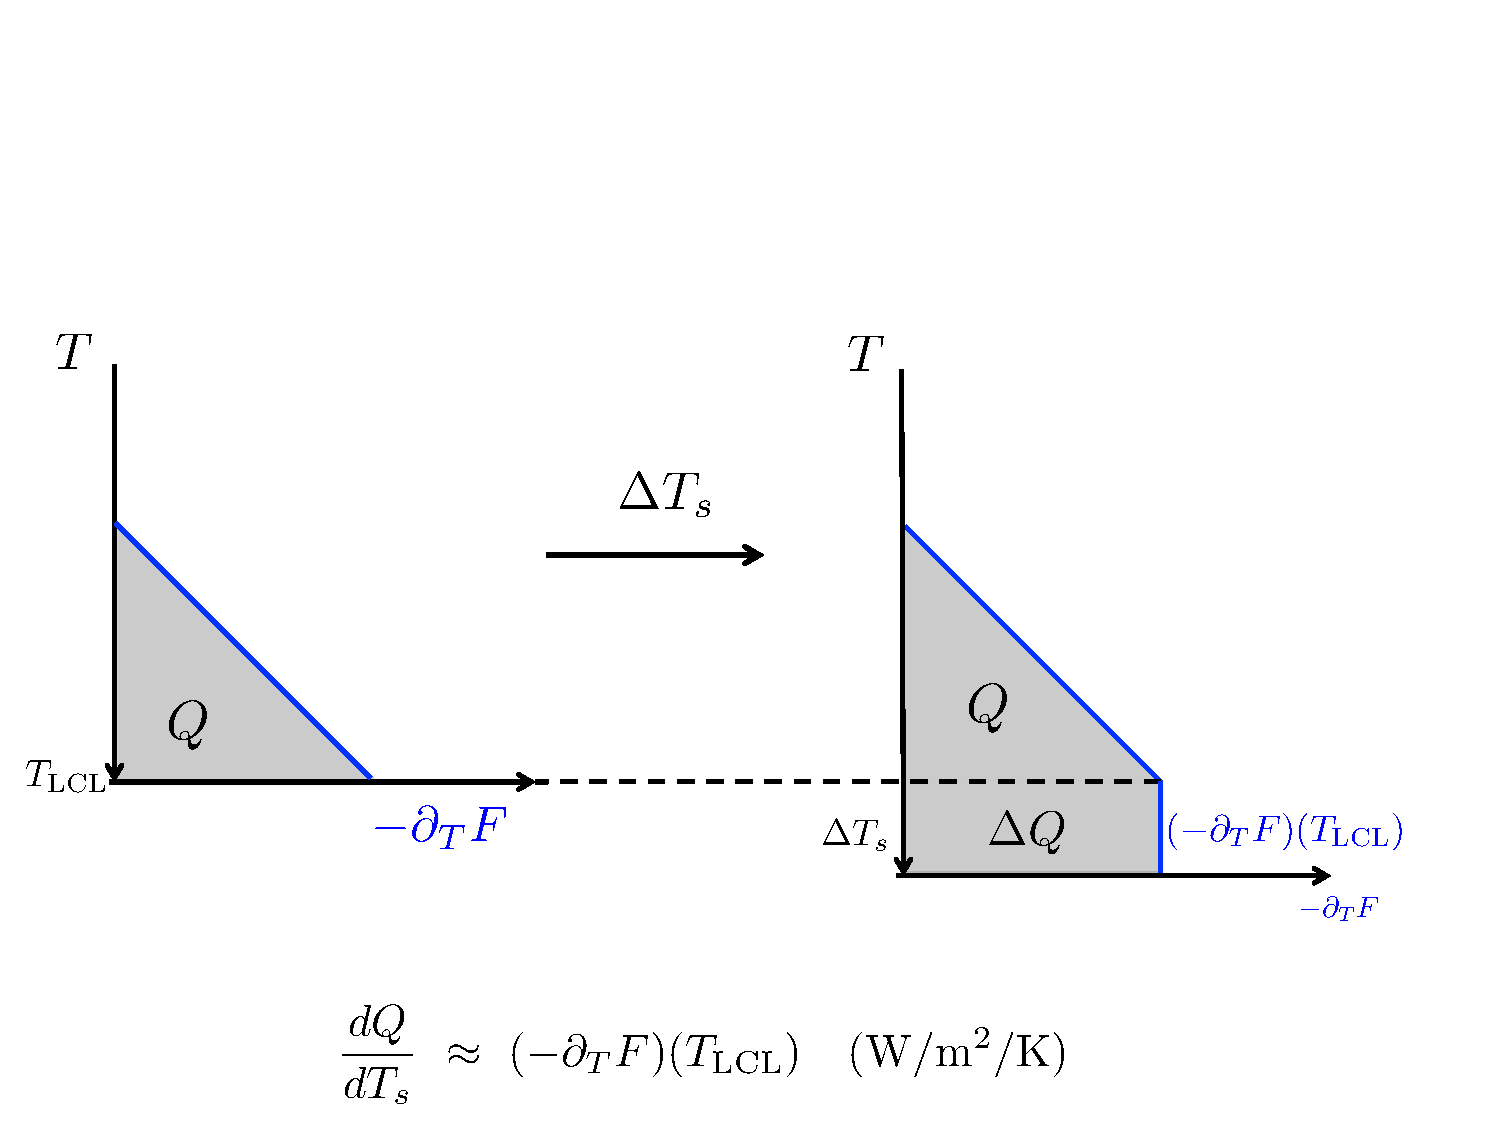
\includegraphics[scale=0.65,trim=0cm 0cm 0cm 5cm,clip=true]{../figures/dqdts_cartoon.pdf}
		\caption{Cartoon depicting the increase in $Q$ with \Ts\ in Eqn. \eqnref{dqdts}. Increasing the temperature range of the troposphere  exposes more of the \Ts-invariant curve $(\ppt F)(T)$ (blue lines). The contribution  of this newly exposed region to column-integrated cooling is given by Eqn. \eqnref{dqdts}.
		\label{dqdts_cartoon}
		}
	\end{center}
\end{figure}


%Figure Qnet_varsst
\begin{figure}[h]
	\begin{center}
			\includegraphics[scale=0.6]{../figures/Qnet_varsst.pdf}
		\caption{Column-integrated cooling $Q$ vs. \Ts\ (black circles), along with slopes $d Q/d \Ts$ (red lines) as diagnosed from \eqnref{dqdts}. These are shown for the SW (left), LW (center) and Net (right) channels.  The black dashed lines connect the black circles and give a benchmark slope against which to compare the red lines. The `Net' panel also gives CRM-diagnosed precipitation values in blue stars. See text for discussion.
		\label{Qnet_varsst}
		}
	\end{center}
\end{figure}

%Figure local_pptf_profiles
\begin{figure}[h]
	\begin{center}
			\includegraphics[scale=0.5]{../figures/local_pptf_profiles.pdf}
		\caption{ Profiles of climatological $-\ppt \Fnet (T)$ from HadGEM2-A for AMIP and AMIP4K simulations, for single columns at various locales. \textbf{Left}: West Pacific warm pool, $\Omega = (135^\circ\ \east, 0^\circ)$  \textbf{Center}: Trade cumulus regime, $\Omega = (210^\circ\ \east, 20^\circ\ \north)$ \textbf{Right}: East Pacific cold tongue, $\Omega = (270^\circ\ \east, 10^\circ\ \south)$
		\label{local_pptf_profiles}
		}
	\end{center}
\end{figure}


%%Figure singlegcm_pptfg_profiles
%\begin{figure}[h]
%	\begin{center}
%			\includegraphics[scale=0.5]{../figures/singlegcm_pptfg_profiles.pdf}
%		\caption{\textbf{Left}: Profiles of $-\ppt \Fgl (T)$, as defined by Eqn. \eqnref{pptfgl_def}, for the SW, LW, and Net channels, for HadGEM-2A. \textbf{Right}: Same as left panel, except in $\alpha$ coordinates rather than $T$ coordinates.
%		\label{singlegcm_pptfg_profiles}
%		}
%	\end{center}
%\end{figure}


%Figure pptfg_profiles
\begin{figure}[h]
	\begin{center}
			\includegraphics[scale=0.6]{../figures/pptfg_net_profiles.pdf}
		\caption{ Profiles of $-\ppt \Fnetgl(\alpha)$ for the six CFMIP models, AMIP and AMIP4K runs.
		\label{pptfg_profiles}
		}
	\end{center}
\end{figure}

%%Figure dqdts_decomp
%\begin{figure}[h]
%	\begin{center}
%			\includegraphics[scale=0.8]{../figures/dqdts_decomp.pdf}
%		\caption{Diagnoses of $d\, (\ln Q)/d\Ts$ using terms I, II, and III from Eqn. \eqnref{dqdts_global}, compared to direct diagnosis from AMIP and AMIP4K model output $Q$.
%		\label{dqdts_decomp}
%		}
%	\end{center}
%\end{figure}
%


\bibliographystyle{apa}
\bibliography{/Users/nadir/Dropbox/bibtex_mendeley/library}


\end{document}

